\documentclass{article}
\usepackage[utf8]{inputenc}
\usepackage{amsfonts}
\usepackage{amsmath}
\usepackage{todonotes}
\DeclareMathOperator*{\E}{\mathbb{E}}
\newcommand{\adv}{x_{adv}}
\newcommand{\X}{\mathcal{X}}
\newcommand{\Y}{\mathcal{Y}}
\newcommand{\D}{\mathcal{D}}
\newcommand{\R}{\mathbb{R}}
\newcommand{\sign}{\text{sign}}
\newcommand{\proj}{\text{proj}}

\begin{document}

\section{Adversarial Examples}
Distributional shifts or black swan events are not the only dangers when deploying machine learning systems. In the real world, there exist people with a wide range of intents, some of whom will act as adversaries, purposefully trying to make systems misbehave. There are many possible reasons for this—perhaps the adversary is designing malware to avoid machine learning malware detection algorithms. Perhaps the adversary wants to design sound files which can give unwanted instructions to voice-recognition systems (e.g., Google Home, Amazon Echo). As machine learning systems become more and more integrated into daily life, the incentives to attack these systems only grow larger over time. 

We define \textit{adversarial attack} against a machine learning system as a technique which causes a machine learning system to misbehave. Often adversarial attacks revolve around the generation of \textit{adversarial examples}, inputs designed to confuse or deceive the machine learning system. The literature around adversarial examples seeks to answer three questions regarding these adversarial attacks and examples. 

\begin{itemize}
    \item First, can we discover potential adversarial attacks and reveal vulnerabilities in our machine learning systems? 
    \item Second, can we train systems to be robust to adversarial attacks?
    \item Third, can our knowledge of these strange failure cases inform our understanding of machine learning systems?
\end{itemize}

\noindent Our approach to introducing this field is as follows. In subsection $\ref{sub:lp}$ we introduce the basic $L_p$ adversarial examples paradigm. In subsections $\ref{sub:fgsm}$ and $\ref{sub:pgd}$, we introduce two classic adversarial attacks, namely the Fast Gradient Sign Method (FGSM) and Projected Gradient Descent (PGD). In subsection $\ref{sub:training}$, we introduce adversarial training, a basic defense against adversarial attacks. In subsection $\ref{sub:prop}$, we discuss two surprising properties of adversarial attacks, specifically their transferability $\ref{subsub:transfer}$ and their existence in the real world $\ref{subsub:real}$. Finally, in subsection $\ref{sub:unforseen}$, we go beyond the $L_p$ paradigm and discuss other adversarial attacks which don't fit in this paradigm.

\subsection{$L_p$ Adversarial Robustness}
\label{sub:lp}

Adversarial examples were first discovered by scientists at Google, who noticed that you could add imperceptible noise to an image classifier and make the classifier change its behavior (see figure \ref{fig:openai_panda}) \cite{szegedy2014intriguing}. To humans, the image looked exactly the same, but to the model, the image had changed tremendously. As further scientists explored this phenomena, their work grew into one of the first adversarial attacks paradigms, the ``$L_p$ adversarial robustness paradigm.'' Within this paradigm, we generate adversarial examples by tweaking existing training examples in a targeted fashion. Moreover, this paradigm requires the adversarial example to be `close' to its corresponding training example. We defined this `closeness' through some norm from the $L_p$ family of norms (aka the $p$-norm). Two common $p$-norms are the $2$-norm, which is just the euclidean distance and the $\infty$-norm, which is simply the maximum over the dimensions.
\todo{Mention that I'm talking about images?}
\begin{figure}
    \centering
    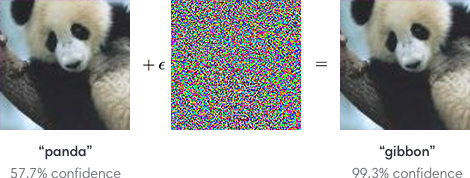
\includegraphics[width=10cm]{images/openai_panda.png}
    \caption{By adding imperceptible noise to an image, we can fool the model into classifying the image improperly.}
    \label{fig:openai_panda}
\end{figure}

We restate the paradigm using mathematical notation. Let $\D$ be a dataset and $x \in \D$ be an example in our training dataset. Let $f: \X \to \Y$ be a machine learning model (usually a classifier) which we are trying to disrupt. An adversarial attack consists of defining a function $g_{adv}: \X \to \X$ which maps training examples to adversarial examples under the constraint that $\|g_{adv}(x) - x\|_p < \varepsilon$. Here $\varepsilon$ represents a `budget' on how far the adversarial example can deviate from the initial training example and is defined before we choose an attack. The stronger the attack, the more drastically $g_{adv}(x)$ changes the behavior of our model $f$, while being close to $x$ (i.e., with $\varepsilon$ being relatively small). With this framework in place, we can start studying some simple adversarial attacks.

\subsection{Fast Gradient Sign Method}
\label{sub:fgsm}

The Fast Gradient Sign Method (FGSM) is one of the earliest techniques in generating adversarial examples \cite{goodfellow2015explaining}. It was developed in 2015 and gained widespread attention within the community for being a simple and quick way to generate adversarial examples. It operates on the $L_\infty$ norm, meaning that each pixel in the images it generates differs at most from the original image by some $\varepsilon$.

Let $l$ be some loss function (e.g., cross entropy loss) used to train $f$. Moreover, let $\hat{y} = f(x)$ be the predictions of our model on input $x$. Then, we can generate adversarial examples as follows:

\[
    \adv = x + \varepsilon * \sign(\nabla_{x}(l(\hat{y},y))).
\]

\noindent The gradient $\nabla_{x}(l(\hat{y},y))$ represents how to modify $x$ to maximize the loss $l(\hat{y}, y)$. We then take the sign of the gradient before adding it to the original example $x$. This does two things. First, it helps bound the gradient between -1 and 1. This bounding of the gradient makes $\adv$ naturally satisfy the $\infty$-norm constraint:

\[
    \adv - x = \varepsilon * \sign(\nabla_{x}(l(f(x),y)).
\]

\noindent Second, taking the sign of the gradient actually works better than naively using the gradient, so long as $f$ can be approximated well as a linear function around the input \cite{goodfellow2015explaining}. Intuitively, taking the sign of the gradient maximally uses up the $\infty$-norm constraint.

In practice, FGSM is a relatively weak method for generating adversarial examples and can be defended against easily. That being said, FGSM often can still deceive models which have not specifically implemented any adversarial defenses. Moreover, FGSM's simplicity makes it a useful baseline attack to expand upon or compare against.

\subsection{Projected Gradient Descent}
\label{sub:pgd}
\todo{Unfinished from here}
After FGSM, we jump to Projected Gradient Descent (PGD), which Madry et al. adapted for adversarial attacks \cite{madry2019deep}. Whereas FGSM was analogous to taking one step of gradient ascent, PGD is analogous to taking multiple steps of gradient ascent. Let $x_i$ represent the adversarial example after $i$ steps of PGD. Let $\alpha$ be a `step size', $\proj$ a function which projects an $x'$ to be within $\varepsilon$ $p$-norm of the original $x$ and $n$ be the total number of steps. Then we repeat the following procedure for $i=1$ to $i=n$:

\begin{align}
    x_{i+1}' &= x_i + \alpha * \nabla_x(l(f(x), y)) \\
    x_{i+1} &= \proj(x_{i+1}')
\end{align}

In practice, PGD generates very strong adversarial examples, as $n$ increases. There are many adversarial defenses which are broken by simply increasing the number of steps, $n$. On the flipside, the strength of PGD's adversarial examples gives us a way to train models to be robust.

\subsection{Adversarial Training}
\label{sub:training}

Now that we've learned about attacks like FGSM or PGD, one natural question might be to ask: ``how might we train models to be \textit{robust} to adversarial attacks?'' One common approach is adversarial training. During adversarial training, we expose our model to adversarial examples and penalize our model if the model is decieved. In particular, an adversarial training loss might be as follows:

\[
    \text{Loss}(f, \D) = \E_{x,y \sim \D}\left[\text{CrossEntropy}(f(x), y) + \lambda \cdot \text{CrossEntropy}(f(g_{adv}(x)), y)\right].
\]

\noindent where $\lambda$ is some hyperparameter determining how much we emphasize the adversarial training. This often reduces accuracy, but increases robustness to the specific adversarial attack which your model is trained on. However, many have shown that robustness towards one type of adversarial attack does not provide robustness to other adversarial attacks. For instance, a model trained on FGSM will not perform well on PGD attacks with $n=10$. PGD was significant because PGD showed that models trained on actually were robust to a whole class of adversarial examples.

\subsection{Properties of Adversarial Examples}
\label{sub:prop}
Adversarial examples also exhibit some special properties. Specifically, adversarial examples are moderately transferable to different models trained on the same dataset (or even on different datasets). Additionally, adversarial examples can be printed out and fool real-world systems through a camera lense. We describe these findings and their implications in this section. 

\subsubsection{Transferability of Adversarial Examples}
\label{subsub:transfer}
First, \cite{szegedy2014intriguing, goodfellow2015explaining} demonstrated that adversarial examples from one model are actually somewhat transferable to other models, including models which were trained on a disjoint training set. The precise accuracy varies depending on attack method, model architecture, and datasets.

This itself has lead to a new type of adversarial attack, which can be performed without access to the actual model. It involves training a surrogate model, attacking that surrogate model, and hoping the attack transfers to the unseen model \cite{papernot2016transferability, papernot2017practical}. 

% Implications

\subsubsection{Real World Adversarial Examples}
\label{subsub:real}

Second, Kurakin et al. demonstrated that adversarial examples can be printed out and fool real-world systems through a camera lens \cite{kurakin2017adversarial}. This serves to demonstrate the adversarial examples are robust to noise and perturbation themselves. Soon after, Brown et al. developed `adversarial patches', paper printouts which can be added to a video feed to attack any image classifiers monitoring the video feed \cite{brown2018adversarial}. Others have designed `toxic signs' which deceive autonomous driving systems \cite{sitawarin2018darts}, stickers which fool facial recognition systems \cite{komkov2021advhat}, and sweaters which fool object detectors \cite{wu2020making}.

% https://github.com/lionelmessi6410/awesome-real-world-adversarial-examples

% Implications

\subsection{Unforseen Attacks}
\label{sub:unforseen}

\todo{Unfinished}
Finally, in recent years, it has been demonstrated that models which are robust according to the ``$l_p$ robustness paraidgm'' still have vulnerabilities when attacked in novel ways. For instance []. To combat this, researchers have tried to generate many different types of novel adversarial attacks []. Moreover, with the variety of adversarial attacks and defenses, it can be difficult to compare them. Recently, there has been work into benchmarking adversarial robustness \cite{croce2021robustbench}. 

% Robust Bench + Unforseen Adversaries.

\bibliographystyle{plain}
\bibliography{reference}

\end{document}
